% --------------------------------------------------------------
% This is all preamble stuff that you don't have to worry about.
% Head down to where it says "Start here"
% --------------------------------------------------------------
 
\documentclass[12pt]{article}

\usepackage{courier}
\usepackage{color}
\usepackage{listings}
\usepackage[square,numbers]{natbib}
\usepackage{tabls}
\usepackage{graphicx}
\usepackage{subcaption}
\usepackage{pdfpages}
\usepackage{mathtools}
\usepackage{enumitem}
\usepackage{hyperref}
\definecolor{dkgreen}{rgb}{0,0.6,0}
\definecolor{gray}{rgb}{0.5,0.5,0.5}




\lstset{language=Matlab,
   keywords={break,case,catch,continue,else,elseif,end,for,function,
      global,if,otherwise,persistent,return,switch,try,while},
   basicstyle=\ttfamily,
   keywordstyle=\color{blue},
   commentstyle=\color{red},
   stringstyle=\color{dkgreen},
   numbers=left,
   numberstyle=\tiny\color{gray},
   stepnumber=1,
   numbersep=10pt,
   backgroundcolor=\color{white},
   tabsize=4,
   showspaces=false,
   showstringspaces=false}
 
\usepackage[margin=1in]{geometry} 
\usepackage{amsmath,amsthm,amssymb}
\usepackage{verbatim}
\usepackage{algpseudocode,algorithm}
\usepackage{setspace}

\newcommand{\lline}{\noindent\makebox[\linewidth]{\rule{\textwidth}{0.4pt}}}
\newcommand{\N}{\mathbb{N}}
\newcommand{\Z}{\mathbb{Z}}
\newcommand{\deriv}[2]{\frac{\mathrm{d} #1}{\mathrm{d} #2}}
\newcommand{\pderiv}[2]{\frac{\partial #1}{\partial #2}}
\newcommand{\bx}{\mathbf{X}}
\newcommand{\ba}{\mathbf{A}}
\renewcommand{\d}{\mathrm{d}}
\newcommand{\upl}{u_{\text{plane}}}
\newcommand{\upt}{u_{\text{point}}}
\newcommand{\D}{\Delta}
\renewcommand{\SS}{\State}
 
\newenvironment{theorem}[2][Theorem]{\begin{trivlist}
\item[\hskip \labelsep {\bfseries #1}\hskip \labelsep {\bfseries #2.}]}{\end{trivlist}}
\newenvironment{lemma}[2][Lemma]{\begin{trivlist}
\item[\hskip \labelsep {\bfseries #1}\hskip \labelsep {\bfseries #2.}]}{\end{trivlist}}
\newenvironment{exercise}[2][Exercise]{\begin{trivlist}
\item[\hskip \labelsep {\bfseries #1}\hskip \labelsep {\bfseries #2.}]}{\end{trivlist}}
\newenvironment{problem}[2][Problem]{\begin{trivlist}
\item[\hskip \labelsep {\bfseries #1}\hskip \labelsep {\bfseries #2:}]\hspace{0.3in}\newline\newline}{\end{trivlist}}
\newenvironment{question}[2][Question]{\begin{trivlist}
\item[\hskip \labelsep {\bfseries #1}\hskip \labelsep {\bfseries #2.}]}{\end{trivlist}}
\newenvironment{corollary}[2][Corollary]{\begin{trivlist}
\item[\hskip \labelsep {\bfseries #1}\hskip \labelsep {\bfseries #2.} ]}{\end{trivlist}}
\newenvironment{problem*}[1][Problem]{\begin{trivlist}
\item[\hskip \labelsep {\bfseries #1} {\hspace{-0.2em}\bfseries:}]}{\end{trivlist}}
\newenvironment{solution}[1][Solution]{\begin{trivlist}
\item[\hskip \labelsep {\bfseries #1} {\hspace{-0.2em}\bfseries:}]\hspace{0.3in}\newline}{\end{trivlist}}
 
\begin{document}
 
% --------------------------------------------------------------
%                         Start here
% --------------------------------------------------------------
 
\title{Programming Assignment 2}%replace X with the appropriate number
\author{Simon Bolding\\ %replace with your name
CSCE 626} %if necessary, replace with your course title
 
\maketitle

\clearpage

%\includepdf[pages={1}]{p1p3.pdf}

\section*{References}

\begin{enumerate}
	\item People in class - Hans Hammer, Daniel Holladay, Josh Hansel
	\item wikipedia.org/wiki/Prefix\_sum,computing.llnl.gov, mpitutorial.com
    \item Class notes
    \item EOS website: sc.tamu.edu/systems/eos
\end{enumerate}

\section{Introduction}

In this work experimental analysis was performed to evaluate the performance
of two different methods for computing prefix sums in parallel: 
algorithm implemented with MPI and an algorithm implemented using OpenMP.  Given a sequence of numbers $x_1, x_2, ..., x_n$, the prefix sums are the partial sums 
\begin{align*}
s_1 =&x_1  \\
s_2 =& x_1 + x_2  \\
\vdots& \\
s_n =& x_1 + x_2 + \cdots + x_n .
\end{align*}
Multiple experiments were performed, and the results were analyzed to compare the performance of the algorithms 
as a function of the number of parallel processors used, for both algorithms.
Coefficients for the theoretical asymptotic complexity were determined. Both strong
and weak scaling studies were performed as well, and speed up studied as a function
of the number of elements. The
algorithms are benchmarked against the best sequential algorithm.

\section{Theoretical Analysis}

\subsection{Sequential Algorithm}

An efficient, time optimal sequential algorithm was used as a reference to
compare to parallel algorithms.  The algorithm is given in Alg.~\ref{alg:1}.
This algorithm has asymptotic time complexity $T(n)=O(n)$, where $n$ is the number of
input integers. Because $n-1$ additions must be performed to calculate the prefix sum,
this is clearly the optimal sequential algorithm. It is noted as an implementation detail that the call to
    \verb{PrefixSumSerial{ uses the same function call in the parallel versions of
        the code.  This ensures there are no optimization differences for this
        function call.
\begin{algorithm}
\begin{algorithmic}
    \caption{Serial prefix sum algorithm\label{alg:1}}
\setstretch{1.1}
\Procedure {PrefixSumSerial}{$A,B$} \Comment{Assumes len($A$)=len($B$)=$n$}
    \State variables: $i$, $n$
    \State $n$ = len($A$)
    \State $B(0)$ := $A(0)$ \Comment{Initialize prefix sum}
    \For{$i=1$ to $n-1$}
        \SS B(i) := A(i)+B(i-1)
    \EndFor
    \Comment{$B$ now contains the prefix sum of $A$}
\EndProcedure
\end{algorithmic}
\end{algorithm}

\subsection{MPI Algorithm}

The algorithm for the MPI implementation is given in Alg.~\ref{alg:mpi}. This
algorithm uses the standard approach from the previous homework of computing local
prefix sums, followed by a global prefix sum on the last element in each local array,
before adding the sum of previous processors to each element. 

The algorithm assumes that the input elements and output prefix elements are
distributed across $p$ processors.  Thus, for $p$ processors and $n$ integers, each
processor contains $m\approx n/p$ elements.  If $n/p$ is not an integer, then the remaining
elements are distributed, one per processor, amongst the first $n\mod p$ elements.  Each processor
computes the prefix sum of its $m$ elements, and order $O(n/p)$ operation.  Using \verb{MPI_Allgather{, a copy of the last
    element in each processor's prefix sum array (representing the sum of all
    elements on each processor) is copied to all processors.  Thus, each processor
    now contains an array $C$ of size $p$, with the $i$-th element containing the sum of the
    elements on the $i$-th processor.  The prefix sum of $C$ is computed by each
    processor, an $O(p)$ operation.  Finally, each processor adds the sum of integers from all previous processors to
    its local prefix sum array as necessary.each processors values.  
    
    For time and work complexity, the initial prefix sums and final value additions
    require $O(n/p)$ time and $O(n)$ work. To perform the global prefix sum, the
\verb{MPI_Allgather{ command was utilized to copy the processor sums to each
    processor. Although $p$ numbers must be communicated, by combining messages in a
    tree-reduction, this command only requires the large communication overhead of
    $O(\log p)$ messages. Thus, as far as asymptotic complexity, this process
    represents an $O(\log p)$ communication time, with $p \log p$ work.  The serial prefix sum of each
    processors array is computed only up to that processor, but this is bounded by an
    $O(p)$ time and $O(p^2)$ work.  Thus, in total, $T(n)=O(n/p+p+log(p))=O(n/p+p)$
    and $W(n)=O(n+p^2+p\log p) = O(n+p^2)$.  It is noted that for the case of the
    experiments performed in this work,
    $n\gg p$, and the $O(p)$ terms become negligible.
    We have verified this
algorithm works in previous homework.


\begin{algorithm}
\begin{algorithmic}
    \caption{MPI prefix sum algorithm\label{alg:mpi}}
\setstretch{1.1}
\Procedure {PrefixSumMPI}{$A$} \Comment{Assumes len($A$)=$n$}
    \State \Comment{Assume $A$ and $B$ distributed evenly on processors, $\approx n/p$ to each processor}
    \State Local variables: $id$, $p$, $m$ \Comment{MPI Rank, number of processors,
    my size}
    \State Local variables: $C,D$ \Comment{Arrays of size $p$ for parallel prefix sum}
    \State $id$ := get\_my\_id() \Comment{Procs. numbered $0,1,\ldots,n-1$}
    \State $m$ := $\lfloor n/p \rfloor$ \Comment{Determine size on each processor}
    \If{$id < n \mod p$}
    \State $m$ :=  $m+1$
    \EndIf
    \State Local variables: $myints$ \Comment{this procs' $m$ input values of $A$}
    \State Local variables: $mypsums$ \Comment{this procs' $m$ prefix sum values of $B$}
    \If{ len($A$) = 1}
        \SS $B(0)$ := $A(0)$
        \SS \textbf{return}
    \Else
        \SS PrefixSumSerial($myints$,$mypsums$)
    \EndIf
    \State MPI\_Allgather($mypsums(m-1)$,$C$) \Comment{$C$ now contains copy of sum
        of elements for \emph{each} of $p$ processors}
    \If{$id>0$}
    $D(0) := C(0)$
    \For{$i=0$ to $id-1$} \Comment{All Procs perform prefix sum on their local copy of $C$}
        \State $D(i)$ := $D(i-1)$+$C(i)$
    \EndFor
        \For{$i=0$ to $n$}
            \SS $mypsums(i)$ := $mypsums(i)$+$D(id-1)$
        \EndFor
    \EndIf \Comment{Collectively the $p$ arrays $mypsums$ contain prefix sum of $A$}
\EndProcedure
\end{algorithmic}
\end{algorithm}

\subsection{OpenMP Algorithm}

The OpenMP algorithm is given in Alg.~\ref{alg:openmp}.  The OpenMP algorithm works similarly to the MPI algorithm above.  Each thread performs the
local prefix sum on its portion of the input array, before a serial prefix sum is
performed on the $p$ processor sums on an additional array.  This step is performed
with the simple serial algorithm by one processor.  This is done because for the
shared memory experiments performed, $p\ll n$, and the memory overhead of using a more
complicated algorithm would ultimately result in a less efficient algorithm run time.  Finally, the sum of previous processor's values are added
to each portion of the array in parallel, as necessary.  

For time complexity, the initial prefix sum and addition of values at the end are
$O(n/p)$, with work complexity $O(n)$.  The prefix sum of the processor sums is
$O(p)$ time, but, because there is shared memory access, this step can be performed
by a single processor.  This results in $O(p)$ work.  In total, for this algorithm,
$T(n)=O(n/p+p)$, where $p\ll n$, and Work is $O(n+p)$. We have verified this
algorithm works in previous homework.

\begin{algorithm}
\begin{algorithmic}
    \caption{OpenMP prefix sum algorithm\label{alg:openmp}}
\setstretch{1.1}
\Procedure {PrefixSumOpenMP}{$A$} \Comment{Assumes len($A$)=$n$}
    \State \Comment{Assume $A$ and $B$ distributed evenly on processors, $\approx n/p$ to each processor}
    \State Local variables: $id$, $p$, $m$ \Comment{MPI Rank, number of processors,
    my size}
    \State Local variables: $C,D$ \Comment{Arrays of size $p$ for parallel prefix sum}
    \State $id$ := get\_my\_id() \Comment{Procs. numbered $0,1,\ldots,n-1$}
    \State $m$ := $\lfloor n/p \rfloor$ \Comment{Determine size on each processor}
    \If{$id < n \mod p$}
    \State $m$ :=  $m+1$
    \EndIf
    \State Local variables: $myints$ \Comment{this procs' $m$ input values of $A$}
    \State Local variables: $mypsums$ \Comment{this procs' $m$ prefix sum values of $B$}
    \If{ len($A$) = 1}
        \SS $B(0)$ := $A(0)$
        \SS \textbf{return}
    \Else
        \SS PrefixSumSerial($myints$,$mypsums$)
    \EndIf
    \State MPI\_Allgather($mypsums(m-1)$,$C$) \Comment{$C$ now contains copy of sum
        of elements for \emph{each} of $p$ processors}
    \If{$id>0$}
    $D(0) := C(0)$
    \For{$i=0$ to $id-1$} \Comment{All Procs perform prefix sum on their local copy of $C$}
        \State $D(i)$ := $D(i-1)$+$C(i)$
    \EndFor
        \For{$i=0$ to $n$}
            \SS $mypsums(i)$ := $mypsums(i)$+$D(id-1)$
        \EndFor
    \EndIf \Comment{Collectively the $p$ arrays $mypsums$ contain prefix sum of $A$}
\EndProcedure
\end{algorithmic}
\end{algorithm}

\section{Experimental Setup}

\subsection{Machine Information}

The parallel programs were tested on \emph{eos}, a machine at Texas A\&M. For all the
results in this work, the available Intel ``Nehalem'' nodes were used. These
processors use Intel 64-bit architecture.  Each node contains two sockets, each
attached to 4 processors, resulting in 8 processing units per core.  There is some potential difference in
memory access times on the chip when going from 4 to 8 cores, where memory must be
accessed off chip.  The nodes are connected in a ``Fat Tree'' topology.  This
results in a constant communication time to access any off board node from any other.

For memory, each core has 32 kB L1 cache and 256 kB of unified L2 cache. Each Nehalem
chip (containing four cores) has an 8 MB shared L3 cache.  There is $\sim 22$ GB of
shared RAM on each node (2 chips, or 8 cores). The RAM has non-uniform access time,
with longer access times when a core accesses the DRAM that is not near it. The RAM
has non-uniform access time, with longer access times when a core accesses the DRAM
that is not near it. More details about the architecture on \emph{eos} can be found
at \url{http://sc.tamu.edu/systems/eos/}

\subsection{Description of Experiments}

Several experiments were performed to gauge the efficiency of the Alg.~\ref{alg:mpi}
and~\ref{alg:openmp}. They are discussed individually below. Batch files to run the
various jobs were created using a Python script.  Output files were processed with a
Python script as well. 

\subsubsection{Strong Scaling Study} 

The purpose of the strong scaling
study is to see how much faster a problem of a fixed size can be solved by
using more processors.  Speed up was used as a performance measure for the strong
scaling study.   Speed up is defined as the ratio $T_{ser}/T_p$, where $T_{ser}$ is the time to solve the problem using the most
efficient serial algorithm and $T_{p}$ is the time to solve the program using $p$
processors with a particular parallel algorithm.  This is different than scalability,
which is the ratio $T_{1}/T_{p}$, which can also be used as a performance measure for
strong scaling.  A program which scales perfectly would show a linear, one-to-one
speed up.  In general this is not the case due to communication and memory overhead.

For both the MPI and OpenMP algorithm, $10^9$ integers was chosen as the input
problem size. The choice of this number was to ensure that the size of each portion of
the input and prefix sum arrays stored by each processor was larger than the $L3$
cache, for all simulations.  The size of the input array for $10^9$ integers is $4$ bytes/int
$\times 10^9$ integers $=4$ GB.  The size of the output arrays, which use 8 byte
longs, is $8\times 10^9$ GB. In total, around $12$ GB of memory is needed, which is well
under the limit of $22$ GB per node.  The largest run of 256 cores still requires
around $10$ MB per core, which is greater than the size of the L3 cache.


\subsubsection{Weak Scaling Study}

A weak scaling study determines the efficiency of the algorithm as you increase the
number of processors, while keeping the problem size \emph{per core} fixed.
The goal of a weak scaling study is to determine the increased cost of an algorithm
as more processors are used to solve a bigger problem.  The metric for the weak scaling studies used was efficiency,
defined as $E = T_p(n)/T_1(n)\times 100\%$, noting that $T_1$ is the time for the parallel
algorithm with not processor, not the time for the serial algorithm.  The ideal
efficiency would be 100\%, resulting in a flat line for $E$ as a function of $p$.

For the weak scaling studies, $10^8$ integers, per core, were used for both the MPI
and OpenMP.  This number was chosen for the same reasons as in the strong scaling
study: the value is larger than the cache size and the total problem size will fit in
the available RAM per node.

\subsubsection{Determining Asymptotic Coefficients}

To determine the validity of our theoretical analysis of the algorithms simulations
were performed for a fixed number of processors with variable input sizes.  This
helps to determine if our theoretical model for run time as a function of input size
and number of processors is sufficiently accurate.  Our model does not account for
communication latencies or memory access times.  It also helps to determine in what
range of problem sizes our asymptotic scalings are accurate.  

The theoretical output time of the model is predicted as $T_{pred}(t)$. In general,
the model $T_{pred}(t)$ is a function of the problem size $n$ and number of processors $p$.
The model can be represented as $T_{pred}(t) = C_0 g(n,p)$ for some $n>n_0$, for a
given system.  By performing experiments for various $n$, given a fixed $p$, the
coefficients of the model $C_0$ and $n_0$ can be determined by plotting the ratio of
the actual to predicted run times.  

For both the OpenMP and MPI algorithm, the dominant term is expected to be $O(n/p)$.
Rather than trying to fit a function to determine the leading coefficients in the
model, which would be difficult due to statistical noise in the results and the small
contribution from the $O(p)$ terms, only the coefficients for the dominant $O(n/p)$
term are determined.  In the case of all algorithms, it is expected
that the $O(n/p)$ term will dominate.



\subsection{Statistics}

The experiments must be repeated to measure various forms of variablity in the
system, e.g., variable communication time, memory access times, inaccuracy of the
timer, etc.  Unless noted otherwise, the experiments were repeated 32 times for each
specific simulations.  The entire program is rerun for each iteration, to ensure the
effect of variability in memory initialization times on exectuion time is represented
accurately.  simulations were performed to
estimate the variability in the system.  The entire simulation was repeated, to
eliminate any unrealistic gains in efficiency due to.

From the 32 simulations, the reported run times are simply the average of the 32
simulations. The standard error in the average of a quantity is $\sigma/\sqrt{N-1}$,
where $\sigma$ is the standard deviation of the quantity.  Since speed up and
scalability are calculated quantities with a statitiscal variance in both terms, it
is necessary to approximate the error in the quantity.  
Based on the standard error propagation formula
(\url{http://en.wikipedia.org/wiki/Propagation_of_uncertainty}), the error for the
ratio of two values is
\begin{equation}
    \sigma \left( \frac{T_i}{T_j} \right) = \frac{T_i}{T_j}
    \sqrt{\left(\frac{\sigma_{T_i}}{T_i}^2\right) + 
    \left(\frac{\sigma_{T_i}}{T_i}^2\right)}
    \label{err}.
\end{equation}
The above equation is used to determine the standard error for all plotted speed ups
and scalability.  The plotted values are the 95\% confidence interval, which is represented, assuming a
Gaussian distribution of the error, as $1.96 \sigma$.

\section{Experimental Results and Analysis.}

Below are given results and discussion for each of the experiments.

\subsection{Strong Scaling Study (speed up)}

The results for the speed up study for the OpenMP is given in
Fig.~\ref{ompsu}. As demonstrated, the algorithm does not demonstrate ideal speedup,
as expected from a non embarrasingly parallel problem, but is able to solve the
problem faster than the optimal serial algorithm.  Some rough timing estimates indicate
that the $O(p)$ calculation in the OpenMP algorithm is $<0.1$ \% of the total runtime
(for 10$^9$ integers), which was on the order of a several seconds.  Thus the limiting
factor is likely the overhead of managing threads and memory access times.  The
algorithm described by Alg.~\ref{alg:openmp} had to be modified slightly to achieve
the shown resolts.  It was modified to allow each thread to create its own memory within the
\verb{omp parallel{ section, for storing the input and prefix sums. This was
        necessary to allow the code to correctly assign memory near the location of
        the cores.  This significantly improved
the speedup, in particular going from 4 to 8 threads, which previously showed a drop
in speedup.  This was the result of processors having to go off chip to access their
portion of the array.  

The speedup results for the MPI algorithm are given in Fig.~\ref{mpisu}. A more
legible plot for the cases of $p\leq16$ is given in Fig.~\ref{mpizoomsu}.  The MPI
algorithm demonstrated better speed up at equivalent counts than the OpenMP
algorithm.  There was much greater variance at 128 and 256 cores, due to much more
off node communication time. 

     \begin{figure}[htbp!]
         \centering
           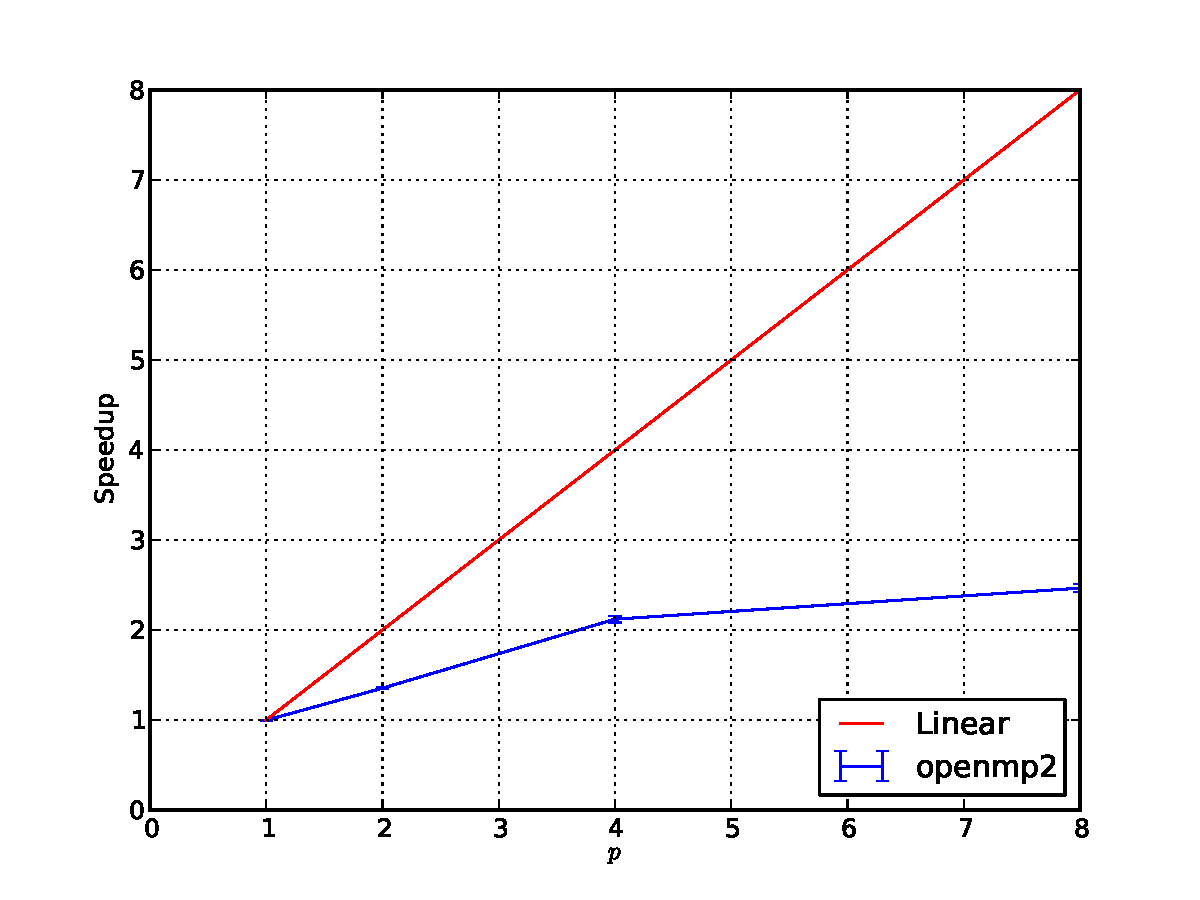
\includegraphics[width=0.75\textwidth]{openmp2_speedup.pdf}
           \caption{Plot of speedup versus $p$ for OpenMP algorithm.\label{ompsu}}
     \end{figure}
\begin{figure}[htbp!]
           \centering
           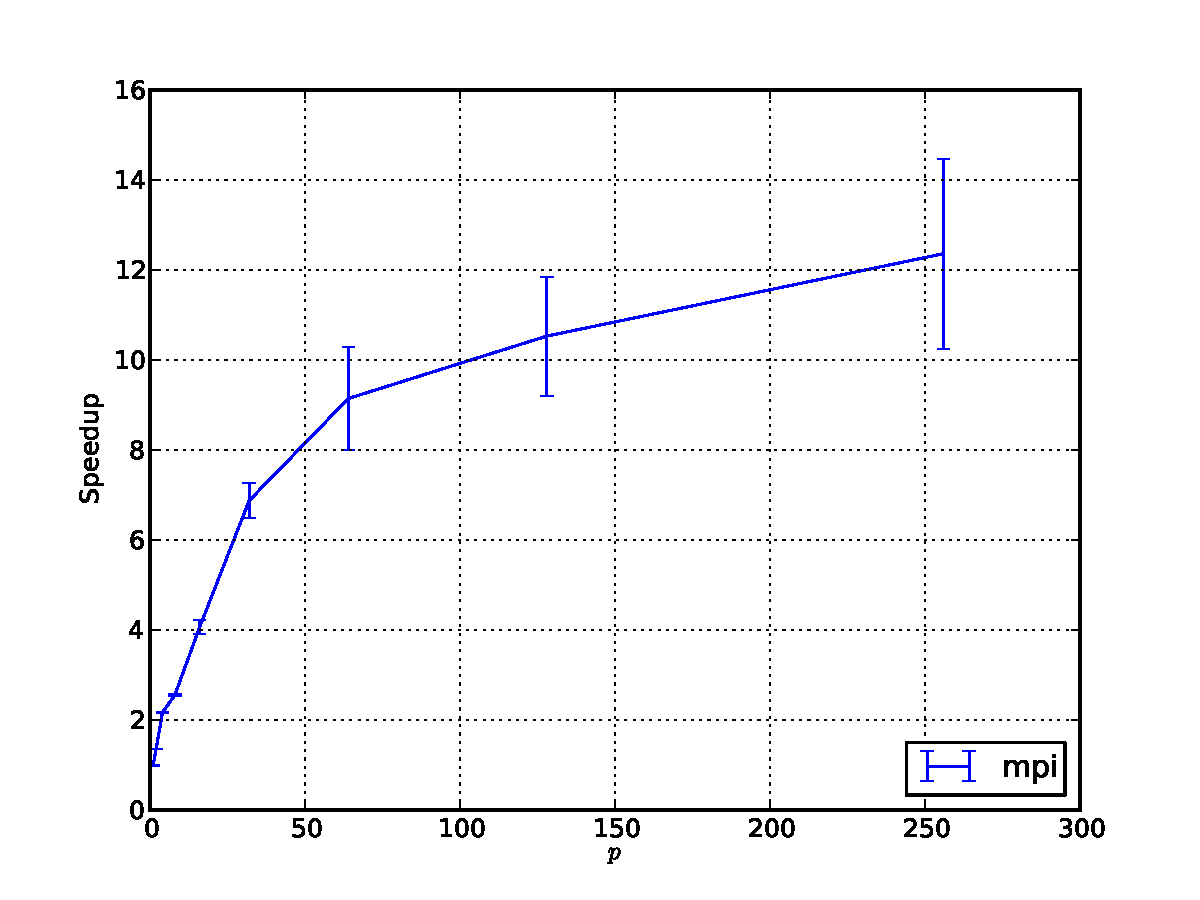
\includegraphics[width=0.75\textwidth]{mpi_speedup.pdf}
           \caption{Plot of speedup versus $p$ for MPI algorithm.\label{mpisu}}
     \end{figure}
\begin{figure}[htbp!]
           \centering
           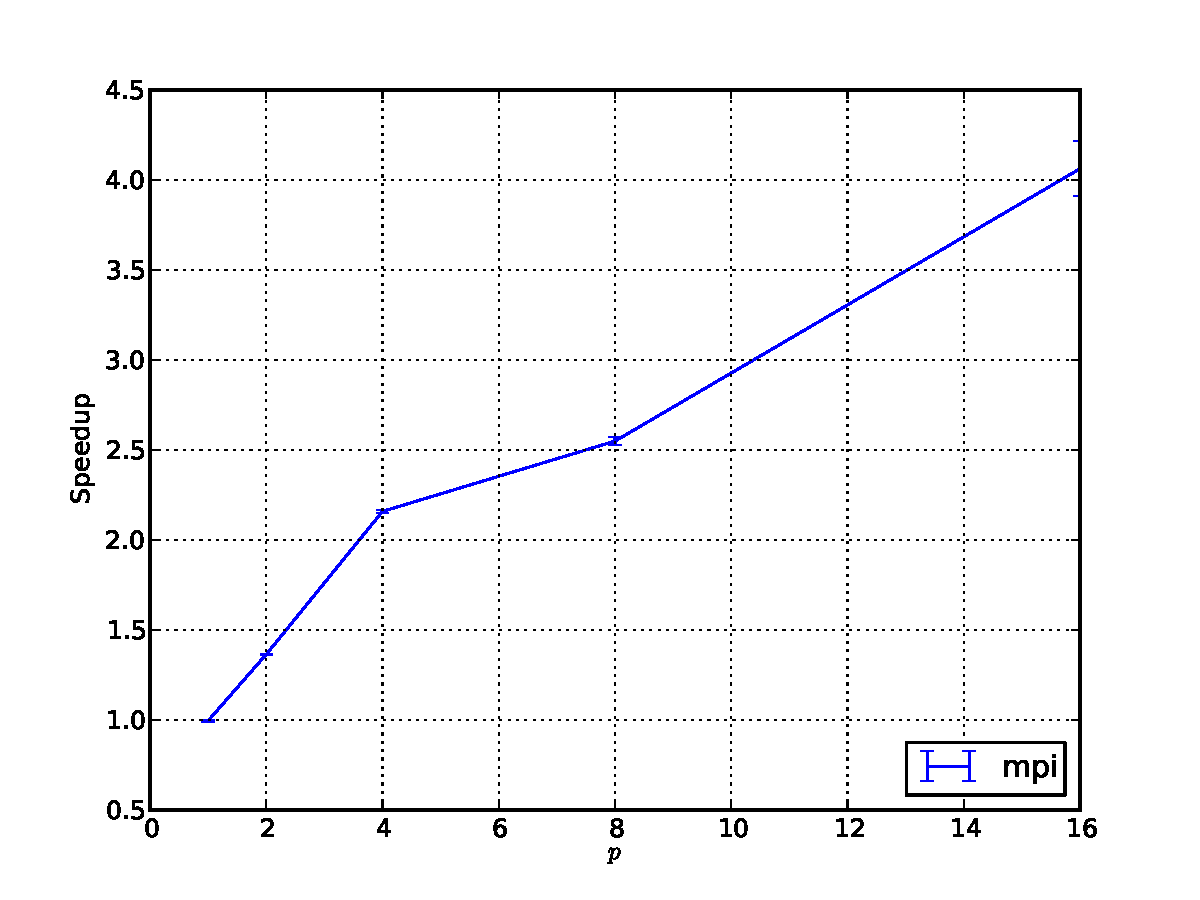
\includegraphics[width=0.75\textwidth]{small.pdf}
           \caption{Zoomed in plot of speedup versus $p$ for MPI
           algorithm.\label{mpizoomsu}}
     \end{figure}




\subsection{Weak Scaling Study}

    It is noted that although
    this algorithm in theory has the same (or slightly worse) time complexity as a linear array approach, there
    is less communication steps, which leads to overall a significantly more efficient algorithm as
    the cost of the communication steps becomes the limiting factor at higher
    MPI rank counts.  This would have similar communication cost to a tree-traversal
    based algorithm.

    OPENMP

To limit memory access overhead
times, it was necessary to allow threads to each have their own memory, rather than
each accessing a portion of the array.  So the algorithm is implemented slightly
different than indicated.   Otherwords the algorithm did not scale well. 

\section{Conclusions}

Since the prefix sum involves such primitive operations, it exposed any memory or
other overhead in computations.  It took very efficient code to demonstraight speed
up.

\end{document}



